% Setup
\graphicspath{./figures}

\chapter{Experimental Evaluation of Service Mesh systems}
\label{chap:experimental-evaluation}

% Introduction
% - What will this chapter contain and what resaarch question it tries to answer

% Prev chapter -> Design of the benchmark and implementation
% This chapter -> Design of experiments, conducting of experiments and results
In the previous chapter (\cref{chap:system-design}), we defined the \gls{sut} and the metrics that are important to evaluate the performance aspects of \gls{sm} systems. This ultimately led to the design, and implementation of \textit{Mesh Bench}, a benchmarking system for \gls{sm} systems. In this chapter, we present the experimental evaluation of \gls{sm} systems using the aforementioned benchmarking tool. With this, we provide an answer to research question \ref{rq-3}. \textit{What are the differences between the different \gls{sm} systems in terms of overhead, throughput and latency?} 


% Rest of the chapter is structured as follows
% - Experimental Setup
% - Experimental Results
% - Analysis/Discussion
The remainder of this chapter is structured as follows. First, in \cref{sec:experiments:design} we introduce the design of the experimental setup. After this, in \cref{sec:experiments:microbenchmarks} we evaluate  and measure the impact of our experimental environment and functional components of our benchmark through several micro benchmarks. Subsequently, in \cref{sec:experiments:results} we present and explain how to interpret the obtained results. Finally, in \cref{sec:experiments:summary} we discuss the results and their implications.

\section{Experiment Design}
\label{sec:experiments:design}

% The goal of the experimental evaluation


The goal of the experimental evaluation is to gain insights into the performance characteristics of \gls{sm} systems. We do this by designing and conducting experiments to extract and gauge relevant metrics for these systems. This section builds upon the knowledge gained in previous chapters and details all the relevant aspects of the experiments.



\subsection{Service Mesh Selection}
\label{sec:experiments:design:meshes}
% What mesh setups did we choose?
% Why did we choose the service meshes included in the experiments?
% None -> Gives baseline
% Linkerd - Most popular (survey results)
% Istio - Most popular (survey results)
% Traefik - Per node arch
% Cilium - ebpf arch

The selection of \gls{sm} systems to include in the experiments is based on two criteria. First, we aimed to include a representative selection of systems that are used in real-world, production grade environments. Secondly, we aim to include systems based on different architectural approaches. In \cref{chap:survey}, we survey the existing state-of-the-art \gls{sm} systems in the industry and have identified the most frequently used, production grade systems. Furthermore, we identified three different architectural styles that could have major implications on the performance of these systems.

With this in mind we present the list of mesh configurations that is used throughout the experiments.

\begin{enumerate}[label=\textbf{SM\arabic*}, leftmargin=3\parindent]
    \item \textbf{None (baseline)}
    \label{exp:sm:0}
    
    To establish a baseline of performance, we start by performing experiments without any \gls{sm} at all. This enables us to not only compare different mesh systems to one another, but also allows us to paint a picture of the performance overhead compared to an unmeshed environment.
    
    \item \textbf{Istio}
    \label{exp:sm:1}
   
    The first mesh of the selection is \textit{istio}, we chose to include this \gls{sm} because of its prevalence in the industry. During our system survey we have identified that \textit{istio} is the most frequently used, production grade system at the time of writing.
    
    \item \textbf{Linkerd}
    \label{exp:sm:2}
   
    The second mesh of the selection is \textit{linkerd}, we chose to include this \gls{sm} because of its popularity. With a service proxy built for \gls{sm} workloads and a focus on performance, this system quickly gained popularity and established itself as a dominant entry in the industry.

    \item \textbf{Traefik}
    \label{exp:sm:3}
    
    The third mesh included in the experiments is \textit{traefik mesh}. We chose to include this mesh because it uses a vastly different architecture for its data plane. During our system survey we established that most of the identified \gls{sm} systems used a per-service proxy. \textit{traefik mesh} was the only system that we identified that used a \textit{per-node} proxy. By including this mesh in our experiments we aim to uncover the performance implications of this type of configuration.
    
    \item \textbf{Cilium}
    \label{exp:sm:4}
    
    The final mesh included in the experiments is \textit{cilium}. A rather new entry in the world of \gls{sm} systems that we chose to include because of its architecture. During our system survey we identified that \textit{cilium} was the only \gls{sm} system which used a \gls{ebpf} based data plane proxy. By including this mesh in our experiments we aim to expose the performance implications such architecture can introduce.

\end{enumerate}


Additionally, in \cref{tab:experiment:design:mesh} we present the versions used for each \gls{sm} during our experiments.

\begin{table*}[t]
\centering

\begin{tabularx}{\linewidth}{llX}

    \toprule
    Service Mesh       & Version & Reason for inclusion \\
    \toprule
    
    Cilium &
    v1.12.0-rc1 &
    The singular identified \gls{sm} system that uses an in-kernel, \textit{eBPF}-based data plane architecture.
    \\
    
    Istio &
    1.14 &
    Prevalence and market share.
    \\
    
    Linkerd2 &
    2.11.2 &
    Prevalence and market share.
    \\
    
    Traefik Mesh&
    1.4.5 &
    The singular identified \gls{sm} system that uses a per-node service proxy in its  data plane architecture.
    \\
    
    \bottomrule
    
\end{tabularx}

\caption[The \gls{sm} systems used in the experiments.]{The \gls{sm} systems used in the experiments and the reason of inclusion.}
\label{tab:experiment:design:mesh}
\end{table*}




\subsection{Metrics}
\label{sec:experiments:design:metrics}
% - System Resources
% - Throughput
% - Latency

To evaluate the performance characteristics of \gls{sm} systems we have to extract relevant metrics from the \gls{sut}. In \cref{chap:system-design}, we designed and implemented a benchmarking instrument to evaluate \gls{sm} systems. During the requirements analysis (\cref{sec:system:requirements-analysis}) we identified the stakeholders, discussed their use cases and formed a list of requirements. During this, we established a set of metrics that are used to evaluate the performance characteristics based on industry best practices.

Below we present the list of metrics used throughout the experiments

\begin{enumerate}[label=\textbf{M\arabic*}, leftmargin=3\parindent]
    \item \textbf{CPU utilization}
    \label{exp:metric:1}
    
    The first metric that we use during the experiments is related to resource utilization. This helps us to establish how much computational overhead the service proxies of a \gls{sm} introduce. All the CPU utilization results are expressed in fractions of a CPU core per second, e.g. the test system has 2 CPU cores and maximum utilization at a given time would be $2.0$. More specifically, we use the \Verb+container_cpu_usage_seconds_total+ as exposed through the \textit{Kubelet} process and obtain the results through \textit{Prometheus} using the query as seen in Listing \ref{lst:promql-cpu}.
    
    \begin{lstlisting}[caption=PromQL query for CPU metric, label=lst:promql-cpu] 
    sum(rate(
        container_cpu_usage_seconds_total{
            container!="",
            pod=~"(target-fortio|traefik-mesh-proxy|cilium).*"
        }[2s]
    )) by (pod, container)
    \end{lstlisting}

    
    \item \textbf{Memory utilization}
    \label{exp:metric:2}
    
    The second metric that we use in the experiments is also related to the resource utilization. We capture the memory utilization of service proxies by measuring the amount of memory they consume during operation. More specifically, we use the \Verb+container_memory_working_set_bytes+ as exposed through the \textit{Kubelet} process and obtain the results through \textit{Prometheus} using the query as seen in Listing \ref{lst:promql-memory}.
    
    
    \begin{lstlisting}[caption=PromQL query for CPU metric, label=lst:promql-memory] 
    sum(rate(
        container_memory_working_set_bytes{
            container!="",
            pod=~"(target-fortio|traefik-mesh-proxy|cilium).*"
        }[2s]
    )) by (pod, container)
    \end{lstlisting}

    
    \item \textbf{Requests per Second}
    \label{exp:metric:3}
    
    The third metric that we use is the amount of requests the system has handled expressed in requests per second. This metrics allows us to identify to measure the amount of throughput or traffic that a system can handle. 

    \item \textbf{Request Latency}
    \label{exp:metric:4}
    
    The fourth metric that we use in our experiments captures the amount of time it takes for a request to be served. This metric, is expressed as latency in milliseconds allows us to establish the overhead caused in the data path of every request in the system.

\end{enumerate}

In the experiments we do not evaluate metrics related to the resiliency of the system. In our requirements analysis we established a requirement to capture this characteristic based on established best practices. However, is not included in the current experimental design. The reason for this is twofold. First of, we uncovered that the \gls{sm} systems handle timeouts and errors in requests differently \cite{linkerd-retry} and that it involves balancing resiliency capabilities and system load. This means that we cannot compare the systems based on their default settings. Second, to create a fair experiment we have to configure these systems to have identical fault tolerance behaviours, which not all systems support. 


\subsection{Workloads}
\label{sec:experiments:design:workloads}
% GRPC Health
% HTTP echo

The selection of workloads aims to represent varying real-world scenarios that a \gls{sm} might encounter. Since a \gls{sm} handles most, if not all the traffic between software services, it can encounter a wide variety of workloads depending on the use case. With this in mind, we design our experiment to use workloads which are as generic as possible. 

During the systems survey conducted in \cref{chap:survey} we analysed the state-of-the-art \gls{sm} systems and identified their key \glspl{fr} and \glspl{nfr}. We identified that \gls{sm} systems handle service traffic in an application aware manner. Furthermore, we identified the most common application level transport protocols in terms of support. With this in mind, we designed the experiments around the two most common application level protocols. 

\subsubsection{HTTP Workload}
\label{sec:experiments:design:workloads:http}

For the experiments that make use of HTTP workloads we use a simple HTTP service. This service represents a simple echo service and replies with the data a client sends to it. This service requires relatively little system resources to operate and scales well to handle large amounts of connections. Additionally, it is also very configurable which enables us to test HTTP workloads with varying conditions and response payloads.

Although this is a synthetic workload which cannot be compared to any real-world workload, it allows us to capture and evaluate the general performance characteristics of \gls{sm} systems under varying circumstances.

\subsubsection{gRPC Workload}
\label{sec:experiments:design:workloads:grpc}

To evaluate how a \gls{sm} performs under varying application level workloads we included a GRPC workload. During the system survey we observed that all the identified \gls{sm} systems supported the \gls{grpc} protocol and noted that it was a common communication standard in distributed computing. With this in mind we introduced a simple \gls{grpc} based workload. To use the \gls{grpc} protocol, both the client and server need to know the service definition\footnote{\url{https://grpc.io/docs/what-is-grpc/core-concepts/\#service-definition}} since this varies from service to service. Best practices dictate that \gls{grpc} based services should to include a health checking endpoint\footnote{\url{https://github.com/grpc/grpc/blob/master/doc/health-checking.md}}. We use this to our advantage by using a simple \gls{grpc} service that includes this endpoint.

This synthetic workload is used to evaluate the performance implications of other (non-HTTP) application level workloads on \gls{sm} systems.

\subsection{Experimental Environment}
\label{sec:experiments:design:environment}
% Create repeatable experiments
% Cluster/Compute Setup
% Metric Collectors

It is important for experiments to be repeatable and that the variance is a little as possible. This allows others to reproduce and verify the results obtained and therefore be of scientific relevance. 

\subsubsection{Cluster Setup}
\label{sec:experiments:design:environment:cluster}

All the experiments were conducted on a \gls{k8s} cluster running on \gls{gcp}. The cluster was created through their managed \gls{k8s} service \gls{gke}. The decision to use their managed service to construct the cluster was based on their flexible, but vast array of network configuration options. In \cref{tab:experiment:design:cluster-config} we present the most important details of the cluster and node configurations used. Which we will now discuss in further detail.

First, we conducted all the experiments in the \textit{europe-west4} region. More specifically, all the compute nodes are located in the \textit{europe-west4-a} data centre location which is located at Eemshaven in the Netherlands. We chose this location as it was closest to our own location. Secondly, we used the most recent version of \gls{k8s} available at the time of writing in the stable release channel. Thirdly, we made use of \textit{VPC-native-routing}\footnote{\url{https://cloud.google.com/kubernetes-engine/docs/concepts/alias-ips}} which implements the \gls{k8s} networking model\footnote{\url{https://kubernetes.io/docs/concepts/services-networking/\#the-kubernetes-network-model}}. Additionally, we disabled \textit{Dataplane V2} an upcoming networking solution based on \textit{cilium} that would conflict with the \gls{sm} systems that we evaluate.

For the node configurations in the cluster we used a single \textit{e2-standard-2} node. This machine has 2 \textit{vCPUs} and 8 GB of memory\footnote{\url{https://cloud.google.com/compute/docs/cpu-platforms}}. We designed the experiments to be run on a single node cluster to abolish any variance in network latencies during the experiments. If for example, we chose to run the load generator on a single node and the target service on another node we introduce additional variance of network latencies.

\begin{table*}[!t]
\centering

\begin{tabular}{l r}


\toprule
\multicolumn{2}{c}{\textbf{GKE Configuration}}       \\
\toprule

\textbf{Compute Region}    & europe-west4            \\
\textbf{Kubernetes Version}& 1.22.8-gke.201          \\
\textbf{Kubernetes Release Channel} & regular        \\
\textbf{VPC-native-routing}         & enabled        \\
\textbf{Dataplane V2}               & disabled       \\

\toprule
\multicolumn{2}{c}{\textbf{Node Configuration}} \\
\toprule

\textbf{Compute Zone}               & europe-west4-a \\
\textbf{Node Count}                 & 1              \\
\textbf{vCPU}                       & 2              \\
\textbf{Memory}                     & 8 GB           \\  

\bottomrule

\end{tabular}


\caption{The cluster configuration used throughout the experiments.}
\label{tab:experiment:design:cluster-config}
\end{table*}

\subsubsection{Metric Collection}
\label{sec:experiments:design:environment:metric-collection}

We capture two types of metrics from the experiments. The first type of metric is related to the load generator (\ref{exp:metric:3}-\ref{exp:metric:4}). These metrics are collected by capturing the \gls{json} output that the load generator produces. The second type of metric is related to resource utilization (\ref{exp:metric:1}-\ref{exp:metric:2}). To analyse the resource overheads of data plane proxies we have to capture the resource overheads at a fine level of granularity, more specifically, at the level of a \gls{pod}.

To collect resource utilization at this level of granularity we bootstrap the cluster with various monitoring instruments. More specifically, we installed \textit{kube-prom-stack}\footnote{\url{https://github.com/prometheus-community/helm-charts/tree/main/charts/kube-prometheus-stack}}, an end-to-end monitoring solution based on the open-source monitoring solution \textit{Prometheus}\footnote{\url{https://prometheus.io/}}.


\subsection{Experiment Variables}
\label{sec:experiments:design:variables}

When performing load testing experiments we can observe and control many of the variables present in the environment. We can do so on three areas of the benchmark. First of, we can control which \gls{sm} is used, this will be done across all experiment. \cref{sec:experiments:design:meshes} details which \gls{sm} configurations are used and why they were chosen. Additionally, we can control the settings of the load generator. This allows us to tweak what kind of loads we can send (\cref{sec:experiments:design:workloads}) but also control how frequent we send loads and how to handle and or wait for responses. The final area which we can tweak is on the side of the target services. The target services are defined as the receiving endpoints of the load generator. This allows us to adjust the way a service responds, allowing us to introduce artificial delays, introduce faults or change payload sizes.

\begin{table*}[!t]
\centering

\begin{tabularx}{\textwidth}{l X r}

% Header
\toprule
\textbf{Variable}    &
\textbf{Description} &
\textbf{Default}     \\
\toprule

% Values
\textbf{Mesh Configuration} &
What type of \gls{sm} configuration is used in the experiment. (\cref{sec:experiments:design:meshes}) &
- \\

\textbf{Workload Type} &
What type of workload the load generator should send (\cref{sec:experiments:design:workloads}). &
HTTP \\

\textbf{RPS} &
How many requests per second the load generator should generate. &
100 \\

\textbf{Connections} &
Number of simultaneous connections to use when making requests. &
32 \\

\textbf{Duration} &
How long the load generator should generate load to the target service before aggregating and outputting results. &
15 minutes \\

\textbf{Payload Size} &
The size of the response payload in bytes. &
0 \\

\bottomrule

\end{tabularx}

\caption[Overview of the experiment variables.]{Overview of the experiment variables.}
\label{tab:experiment:design:exp-variables}
\end{table*}


In \cref{tab:experiment:design:exp-variables} we present the variables that we control across the experiments in this thesis. Additionally, it includes the default values that were used for these variables if they are not introduced as factor variables within an experiment.

\subsection{Experiments}
\label{sec:experiments:design:overview}

We now introduce the four experiments that were designed and used to evaluate the performance characteristics of \gls{sm} systems. For each of the experiments we introduce their primary goal, discuss how they are executed and reason why we chose this particular design. Additionally, \cref{tab:experiment:design:overview} presents an overview of all the experiments, what type of workloads they use, which  metrics they capture and which factors  are used to control the experiment.

\begin{table*}[!t]
\centering

\begin{tabularx}{\textwidth}{l l l X}

% Header
\toprule
\multicolumn{4}{c}{\textbf{Experiment Overview}} \\
\toprule

% Second Header
\textbf{Experiment}     &
\textbf{Workload}       &
\textbf{Metrics}        &
\textbf{Factors}        \\
\midrule

% Experiments
% \textbf{\ref{exp:design:1}} &
\textbf{EXP 1} &
HTTP                        &
\ref{exp:metric:1}, \ref{exp:metric:2}, \ref{exp:metric:3}, \ref{exp:metric:4}         &
\begin{tabular}{@{}l@{}}
    \textbf{Mesh Configuration} \\
    {}
\end{tabular}
\\
\midrule

% \textbf{\ref{exp:design:2}} &
\textbf{EXP 2} &
HTTP                        &
\ref{exp:metric:1}, \ref{exp:metric:2}, \ref{exp:metric:4}         &
\begin{tabular}{@{}l@{}}
    \textbf{Mesh Configuration} \\
    \textbf{RPS} \textit{(1, 100, 500, 1000)} \\
\end{tabular}
\\
\midrule

% \textbf{\ref{exp:design:3}} &
\textbf{EXP 3} &
HTTP                        &
\ref{exp:metric:1}, \ref{exp:metric:2}, \ref{exp:metric:4}         &
\begin{tabular}{@{}l@{}}
    \textbf{Mesh Configuration} \\
    \textbf{Payload Size} \textit{(0, 1kb, 10kb)} \\
\end{tabular}
\\
\midrule

% \textbf{\ref{exp:design:4}} &
\textbf{EXP 4} &
gRPC                        &
\ref{exp:metric:1}, \ref{exp:metric:2}, \ref{exp:metric:3}, \ref{exp:metric:4}         &
\begin{tabular}{@{}l@{}}
    \textbf{Mesh Configuration} \\
    {}
\end{tabular}
\\
\midrule


      

\end{tabularx}


\caption[Overview of the experiments.]{Overview of the experiments, their metrics and factors.}
\label{tab:experiment:design:overview}
\end{table*}

\begin{enumerate}[label=\textbf{EXP\arabic*}, leftmargin=3\parindent]
    \item \textbf{HTTP Maximum Throughput}
    \label{exp:design:1}
    
    \textbf{Goal} \\
    To find the maximum throughput each of the meshed configurations can achieve.
    
    \textbf{Methodology} \\
    The load generator will run in an unrestricted mode and generate as much load as possible without holding back and without any request timeouts. The maximum throughput is determined by looking at the actual number of requests per second in the configuration was able to achieve.
    
    \textbf{Reasoning} \\
    This experiment will serve as a baseline to determine the maximum throughput of all meshed configurations. The results will be used to determine sensible defaults for the experiments with a pre-defined constant throughput.

    \item \textbf{HTTP Constant Throughput}
    \label{exp:design:2}
    
    \textbf{Goal} \\
    To evaluate how \gls{sm} configurations behave under varying levels of load.
        
    \textbf{Methodology} \\
    The load generator will generate load in a constant and uniform throughput setting. This means that the load generator will produce a set number of requests per second and will not deviate or try to catch up when requests are not processed in time.
    
    \textbf{Reasoning} \\
    This experiment evaluates the \gls{sm} configurations under similar levels of load. This allows us to compare these configurations to one another when they undergo the same workloads.
    
    \item \textbf{HTTP Payload}
    \label{exp:design:3}
    
    \textbf{Goal} \\
    To evaluate how \gls{sm} configurations behave with varying payload sizes.

    \textbf{Methodology} \\
    The load generator will produce HTTP requests to the target service, which in turn will respond with pre-determined payload sizes.

    \textbf{Reasoning} \\
    This experiment introduces several pre-determined payload sizes to evaluate the effects of additional application data being transferred in meshed environments. This allows us to study the effects and potential additional overheads extra data transfers may cause. 
        
    \item \textbf{gRPC Maximum Throughput}
    \label{exp:design:4}
    
    \textbf{Goal} \\
    To evaluate how meshed configurations behave with alternative communication protocols.
        
    \textbf{Methodology} \\
    The load generator will generate gRPC traffic towards the gRPC service and do so in an unrestricted manner, meaning it will try to generate as much load as possible without holding back and without enforcing any timeouts. The maximum throughput is determined by looking at the actual number of requests per second in the configuration was able to achieve.
    
    \textbf{Reasoning} \\
    This experiment allows us to evaluate the effects of alternative application level protocols. During the system survey we uncovered that \gls{sm} systems inspect and use this data to for both observability and routing functionalities. This experiment allows us to uncover the effects of alternative, but common, application level protocols widely used within the industry.

\end{enumerate}


\section{Microbenchmarks}
\label{sec:experiments:microbenchmarks}

Before conducting our designed experiments, we evaluate our experimental setup through several micro benchmarks. The goal of these benchmarks is to measure the impact of our functional benchmark components and experimental environment.


\subsection{Measuring the impact of a multi-node setup}
\label{sec:experiments:microbenchmarks:node-count}

The first micro benchmark that we have conducted compares two experimental environments. In \cref{sec:experiments:design:environment}, we introduced our experimental environment and discussed the cluster configuration that we have use for our experimental evaluation. We discussed that we designed the experiments to be run on a single node cluster to abolish any variance in network latencies. However, this also implies that the benchmark system is running on the same node and this can have an effect on the results of the experiments.

To evaluate the impact of such a cluster configuration we constructed a micro benchmark. In this micro benchmark, we perform an experiment similar to the design of \ref{exp:design:1}, in which we try to find the maximum throughput of our experimental environment. In this experiment, however, we only perform it on an unmeshed (baseline) configuration to simplify and limit any variance a \gls{sm} system can impose and run it for a total duration of 15 minutes. We compare two experimental environments, in which we change the cluster configuration. The first environment has a single node cluster which runs the benchmark system and the target services. The second environment has a two node cluster, one of these nodes runs the benchmark system whereas the other node runs the target service.


\begin{figure}[!t]
    \centering
    
    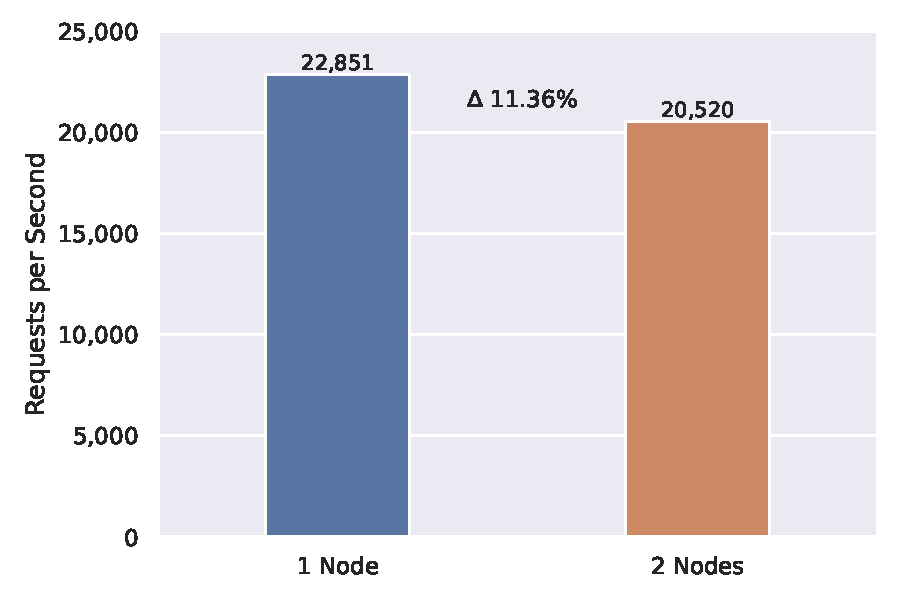
\includegraphics[width=0.8\linewidth]{5_experimental_evaluation/figures/microbench-node-count.pdf}

    \caption[Micro benchmark - Comparing the average maximum throughput of two cluster configurations]{Comparing the average maximum throughput of two cluster configurations.}
    
    \label{fig:microbench:node-count}
\end{figure}

The results of the micro benchmark can be seen in \cref{fig:microbench:node-count}. The environment using a single node reached an average throughput of 22851 requests per second over the duration of the 15-minute experiment. The environment using two nodes, however, only managed to reach 20520 requests per second. Although the benchmarking system in the two node environment has more system resources to work with, it was unable to reach the throughput levels of the single node environment. Therefore, we can conclude that the experimental environment using one node does not cause any system resource related bottlenecks and that our proposed design using one node is a valid approach for our experiments.


\subsection{Measuring the impact of the impact of our target service}
\label{sec:experiments:microbenchmarks:target-svc}

The second micro benchmark that we conduct tries to establish if the target services can be the cause of a bottleneck during our experimental evaluation. As discussed in our analysis of the \gls{sut} (see \cref{sec:system:sut}), we measure the data path towards our service to evaluate the overheads of a \gls{sm} system and its proxy architecture. However, to evaluate this, we need to emulate a software service that acts as a purely functional component in our benchmark. In our prototype implementation of \textit{Mesh Bench}, we use a simple HTTP and gRPC service (see \cref{sec:system:implementation}). 

To determine if the target service implementation can be the cause of a bottleneck, we used a different workload generator than the one we use for our benchmarking system. Although \textit{fortio} has a flexible feature set and is highly configurable, \textit{wrk2} (as discussed as alternative in \cref{sec:system:implementation}) was the most performant workload generator we have evaluated and can generate more load than the other systems mentioned. During our micro benchmark, we generate several levels of load beyond that of our designed experiments, to make sure that the target service is not a bottleneck in any of the results.

\begin{figure}[!t]
    \centering
    
    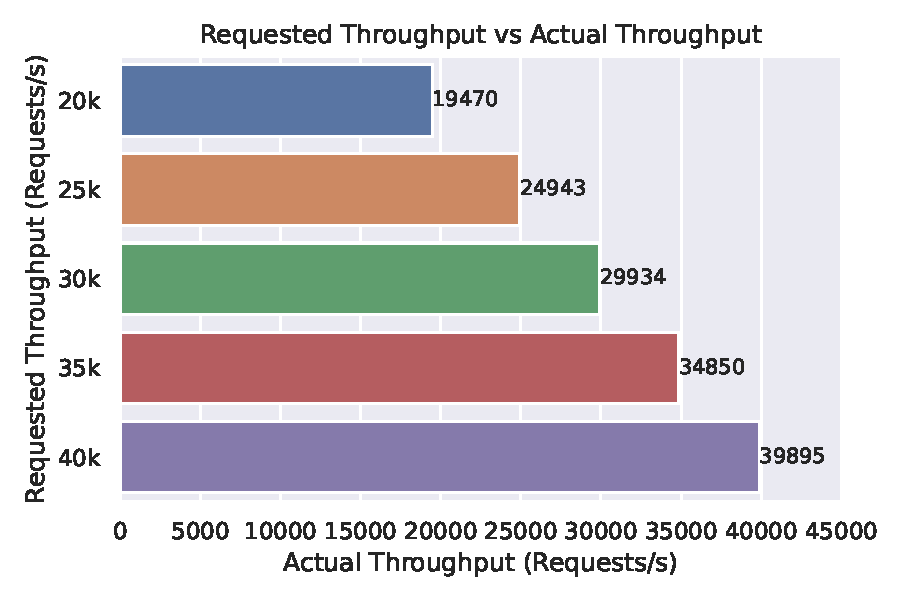
\includegraphics[width=0.8\linewidth]{5_experimental_evaluation/figures/microbench-target-service.pdf}

    \caption[Micro benchmark - Measuring the maximum throughput levels of the target service]{Measuring the maximum throughput levels of the target service.}
    
    \label{fig:microbench:target-svc}
\end{figure}

In \cref{fig:microbench:target-svc} we present the results of the micro benchmark. This chart shows the requested throughput of the workload generator on the y-axis and shows the actual throughput of successful requests on the x-axis. From these results, we can derive that the target services had no problems handling the levels of throughput generated as the actual throughput levels are very close to the requested levels. Note that these levels of throughput exceed the maximum throughput of the experiment results as discussed in the next section, which shows that the target service as functional component in our benchmark system is not the cause of any bottlenecks.

\section{Experiment Results}
\label{sec:experiments:results}

In this section, we present the results obtained from the experiments as defined in \cref{sec:experiments:design:overview}. We first present the main findings in \cref{sec:experiments:main-findings}. After this, we present and explain how to interpret the results per experiment and discuss their findings in greater detail.


\subsection{Main Findings}
\label{sec:experiments:main-findings}
% Significant decrease in throughput
% Additional avg latency, esp tail ends. p99+
% Traefik experiences bottlenecks, bimodal distribution
% Istio consumes most CPU resources
% Applications Payloads seem to have little effect on performance
% Application protocol seems to have little impact, although linkerd performs a bit worse on gRPC throughput
% Traefik failed to handle gRPC worklaods
% Cilium best allround performer

We now present the main findings of the conducted experiments.

% \begin{enumerate}[label=\textbf{MF\arabic*}, leftmargin=3\parindent]
%     \item \textbf{There can be a significant drop in maximum throughput when using a service mesh}
%     \label{exp:mf1}
%     Every service mesh suffers from a decrease in maximum throughput. The observed decrease in throughput varies greatly, with a best-case scenario having a  $-16.8\%$ decrease while the worst performing configuration has a significant  $-97.38\%$ decrease in maximum throughput.
    
%     \item \textbf{There can be a significant increase in request latencies when using a service mesh}
%     \label{exp:mf2}
%     A service mesh introduces additional request latency by introducing a network proxy in front of the service. This additional overhead, however, can have a large impact on average and tail end request latencies as observed. With the best performing mesh increasing the average request latency with $20.27\%$ whereas the worst performing configuration saw a staggering $3720.95\%$ uplift.
    
%     \item \textbf{Traefik mesh experiences bottlenecks after it reaches a certain throughput threshold}
%     \label{exp:mf3}
%     We observed that \textit{Traefik} cannot perform above a certain throughput level, and will throttle requests, resulting in a bimodal distribution of request latencies and a significant loss of performance for those requests.
    
%     \item \textbf{Istio is the most demanding in terms of CPU utilization}
%     \label{exp:mf4}
%     We observe that \textit{Istio} consumes significantly more CPU resources compared to other configurations. We also observe that this is due to its data plane proxy which does not scale as well as the proxies in other configurations.
    
%     \item \textbf{Application payloads have little to no effect on the observed performance}
%     \label{exp:mf5}
%     We observed that increasing the application payload, has little to no effect on the performance of meshed configurations.
    
%     \item \textbf{Application level protocols have little to no effect on the observed performance}
%     \label{exp:mf6}
%     We observed that different layer 7 protocols, HTTP vs gRPC, had little to no impact on the decrease in throughput observed.
    
%     \item \textbf{Traefik was unable to handle gRPC workloads}
%     \label{exp:mf7}
%     We observed that \textit{Traefik} was unable to handle and execute gRPC workloads in our experiments even though it listed explicit support for gRPC.
    
%     \item \textbf{Cilium was the best all-round performing configuration, with a significant margin}
%     \label{exp:mf8}
%     We observed that the configuration using \textit{Cilium} outperformed any other configuration using a \gls{sm} with significant margins in all the experiments that were conducted.
% \end{enumerate}

\begin{enumerate}[label=\textbf{MF\arabic*}, leftmargin=3\parindent]
    \item \textbf{Using a \gls{sm} can lead to a significant decrease in sustained throughput.} 
    \label{exp:mf1}
    
    \textit{Observed in:} \ref{exp:design:1} -  \cref{sec:experiments:results:per-experiment:01}
    
    \item \textbf{There is a significant variance in the amount of sustained throughput that \gls{sm} systems can handle.}
    \label{exp:mf2}
    
    \textit{Observed in:} \ref{exp:design:1} -  \cref{sec:experiments:results:per-experiment:01}

    \item \textbf{The network latency overhead caused by the proxy of Cilium is minimal.} \textit{as observed in:} \ref{exp:design:1}
    \label{exp:mf3}
    
    \textit{Observed in:} \ref{exp:design:1} -  \cref{sec:experiments:results:per-experiment:01}
    
    \item \textbf{The latencies observed from Istio under load have a large spread, and especially suffer in their tail end.}
    \label{exp:mf4}
    
    \textit{Observed in:} \ref{exp:design:1} -  \cref{sec:experiments:results:per-experiment:01}
    
    \item \textbf{Traefik mesh performs an order of magnitude worse than any other evaluated service mesh in terms of request latencies when the system is under full load.}
    \label{exp:mf5}
    
    \textit{Observed in:} \ref{exp:design:1} -  \cref{sec:experiments:results:per-experiment:01}
    
    \item \textbf{Traefik experiences bottlenecking behaviour under a load of approximately 500 requests per second resulting in a bimodal distribution of request latencies.}
    \label{exp:mf6}
    
    \textit{Observed in:} \ref{exp:design:2} -  \cref{sec:experiments:results:per-experiment:02}
    
    \item \textbf{There can be a significant difference in the amount of CPU utilization for different \gls{sm} systems under similar levels of load.}
    \label{exp:mf7}
    
    \textit{Observed in:} \ref{exp:design:2} -  \cref{sec:experiments:results:per-experiment:02}
    
    \item \textbf{The memory footprint of data plane proxies is negligible and does not significantly increase under higher levels of throughput.}
    \label{exp:mf8}
    
    \textit{Observed in:} \ref{exp:design:2} -  \cref{sec:experiments:results:per-experiment:02}
    
    \item \textbf{The size of the application payload does not have a significant effect on the performance of data plane proxies and resource utilization levels.}
    \label{exp:mf9}
    
    \textit{Observed in:} \ref{exp:design:3} -  \cref{sec:experiments:results:per-experiment:03}
    
    \item \textbf{The configuration using Traefik was unable to process any gRPC based requests.}
    \label{exp:mf10}
    
    \textit{Observed in:} \ref{exp:design:4} -  \cref{sec:experiments:results:per-experiment:04}
    
    \item \textbf{Both gRPC and HTTP-based workloads experience similar reductions in terms of sustained throughput.}
    \label{exp:mf11}
    
    \textit{Observed in:} \ref{exp:design:4} -  \cref{sec:experiments:results:per-experiment:04}
 
\end{enumerate}

% Results per experimetn
\subsection{\textbf{EXP 1} - HTTP Maximum Throughput}
\label{sec:experiments:results:per-experiment:01}
% Goal:
% To find the maximum throughput each of the meshed configurations can achieve.


The first experiment evaluates the \gls{sm} systems when they are fully satiated, i.e. they are at full capacity and handling the maximum amount of load that they can process. This amount of load, or throughput, is measured by the number of requests per second the system can process.


\subsubsection{Maximum Sustained Throughput Analysis}
\label{sec:experiments:results:per-experiment:01:throughput}

In \cref{fig:exp:01:maximum-throughput} we present a bar chart which depicts the average, sustained throughput that a \gls{sm} system was able to process throughout the duration of the experiment. On the y-axis we present the different \gls{sm} configurations, whereas the x-axis represents the throughput in requests per second. Next to each bar we present the actual observed value and the percentage of throughput a system was able to process compared to the  best performing configuration, which in this case is the baseline.


\begin{figure}[t]
\centering
\makebox[\textwidth][c]{
    \begin{minipage}{.65\textwidth}
      \centering
      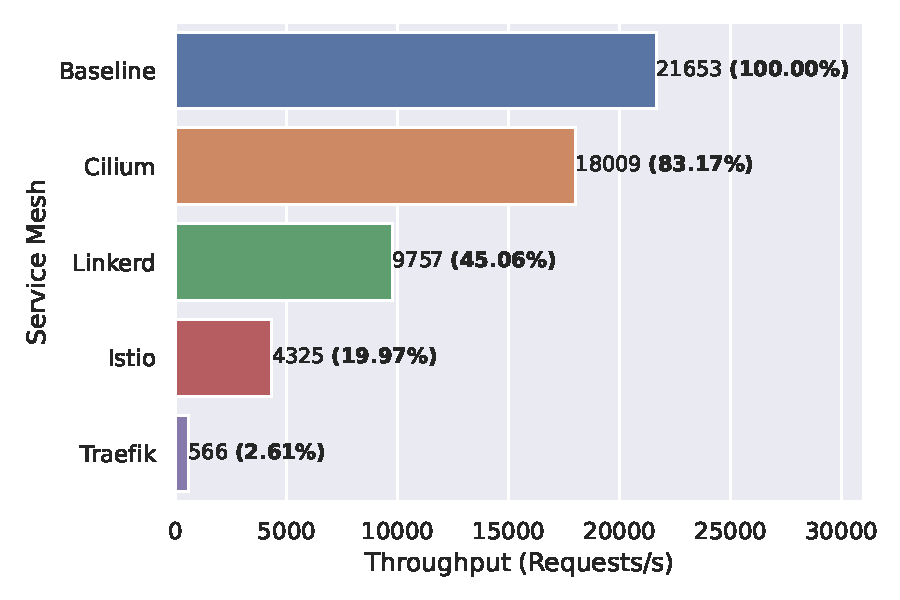
\includegraphics[width=\linewidth]{5_experimental_evaluation/figures/exp-01-max-throughput.pdf}
      \caption[Experiment 1 - Average throughputs of \gls{sm} systems under maximum load.]{Average throughputs of \gls{sm} systems under maximum load.}
      \label{fig:exp:01:maximum-throughput}
    \end{minipage}
    
    
    \begin{minipage}{.65\textwidth}
      \centering
      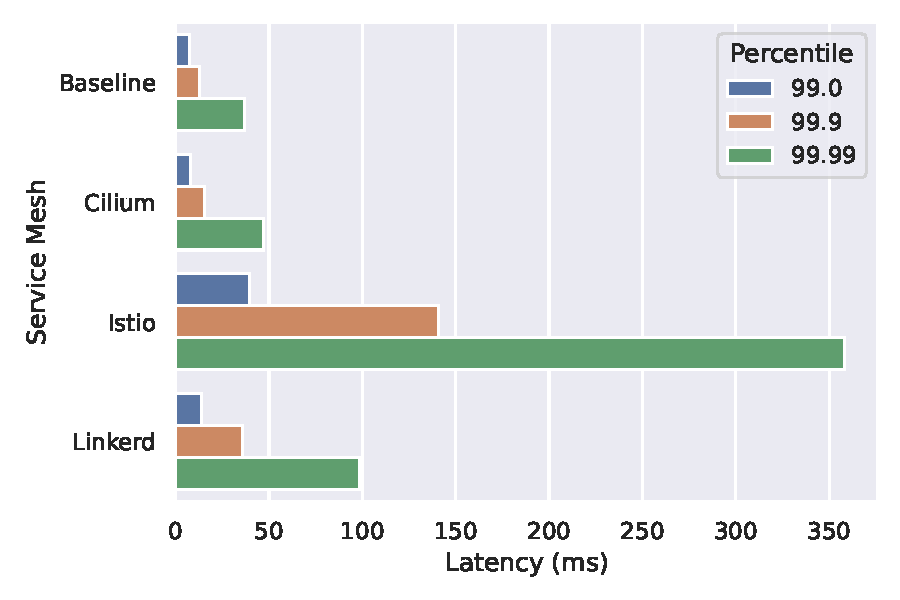
\includegraphics[width=\linewidth]{5_experimental_evaluation/figures/exp-01-tail-latencies.pdf}
      \caption[Experiment 1 - Tail end latencies of \gls{sm} systems under maximum load.]{Tail end latencies of \gls{sm} systems under maximum load.}
      \label{fig:exp:01:tail-end-latencies}
    \end{minipage}
}
\end{figure}


From these results, we can derive that all the \gls{sm} systems experience a loss of throughput compared to the baseline configuration. We can relate this observation to the fact that the \gls{sm} systems introduce additional components in the form of proxies in the critical data path of requests. Every request has to be processed by these proxies, which in turn leads to the decrease in maximum sustained throughput. However, even through the decrease in throughput is expected, the amount of this decrease is rather significant. Cilium is the best performing \gls{sm} configuration in this experiment in terms of throughput. However, it still experienced a massive $16.83\%$ reduction compared to the baseline configuration. This observation leads to our first main finding: 

\begin{shaded*}
    \noindent
    \textbf{MF1}: 
    Using a \gls{sm} can lead to a significant decrease in sustained throughput.
\end{shaded*}

Another observation we can make from these results is the amount of variance there is among the evaluated \gls{sm} systems. We already established that Cilium is the best performing \gls{sm} system in terms of throughput, even though it had a significant reduction compared to the baseline configuration. This reduction in throughput, however, is little compared to the performance of other configurations. The configuration using Linkerd led to a $54.94\%$ reduction and Istio saw a staggering $80.09\%$ reduction in throughput. The worst performing configuration was using Traefik. This configuration only managed to serve a tiny fraction of the requests and experienced a massive $97.39\%$ reduction in throughput compared to the baseline configuration. From these observations, we can conclude that there is a large variance in the observed throughputs among \gls{sm} systems, where the reductions in throughput range from $16.83\%$ to $97.39\%$. This leads to our second main finding:

\begin{shaded*}
    \noindent
    \textbf{MF2}: 
    There is a significant variance in the amount of sustained throughput that \gls{sm} systems can handle.
\end{shaded*}

\subsubsection{Latency Analysis}
\label{sec:experiments:results:per-experiment:01:latency}

In our previous analysis we looked at the amount of requests a configuration can handle. In this part of the analysis we take a look at the durations of the requests themselves. We measure the latency of each request. These latencies represent the time it takes for a request to complete. This is measured from the moment the workload generator sends a request until it successfully receives a response from the target service.

To fully understand the impact that the values and distributions in this analysis can have on real-world application performance, we have to refer to the manner in which applications are often constructed. When using a service-oriented architecture, and namely one using the granularity of microservices, you create an application of many interconnected services. Applications can consist of thousands of microservices \cite{design-example-microservices, netflix-microservices-cost} and a user can indirectly use hundreds of backing services. To evaluate latencies in such a model, we follow the practices as described in the works of Gil Tene \cite{Tene2015-measure-latency}. Because of this model, the tail end latencies are more common than one might expect due to the nature of probabilities. As an example, the ~99.995th percentile of latencies will be experienced in a procedure involving 200 microservices in more than 99\% of the time. 


\begin{figure}[t]
\centering
\makebox[\linewidth][c]{
    \begin{subfigure}{.65\textwidth}
      \centering
      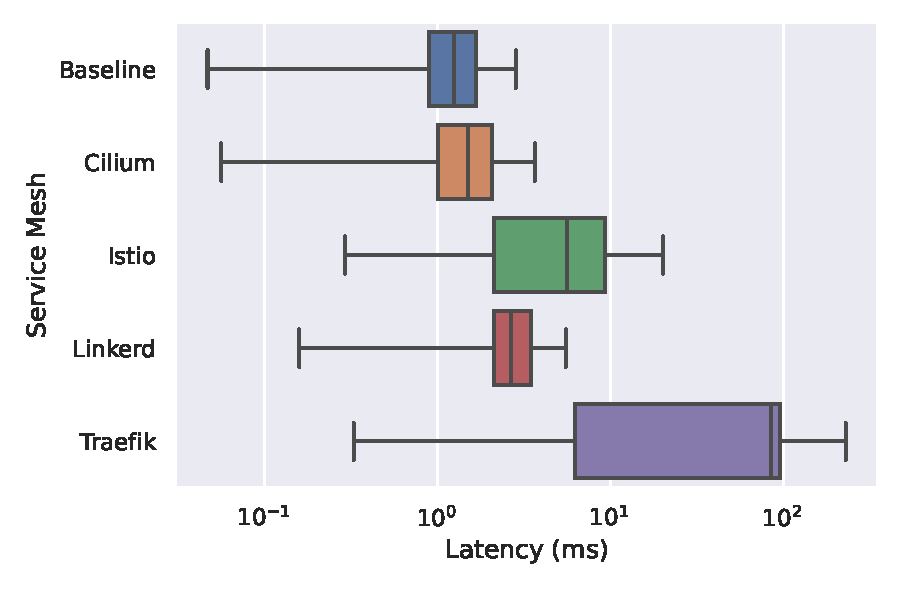
\includegraphics[width=\textwidth]{5_experimental_evaluation/figures/exp-01-latency-log.pdf}
      \caption{Logarithmic scale}
      \label{fig:exp:01:boxplots-latency:log}
    \end{subfigure}
    
    
    \begin{subfigure}{.65\textwidth}
      \centering
      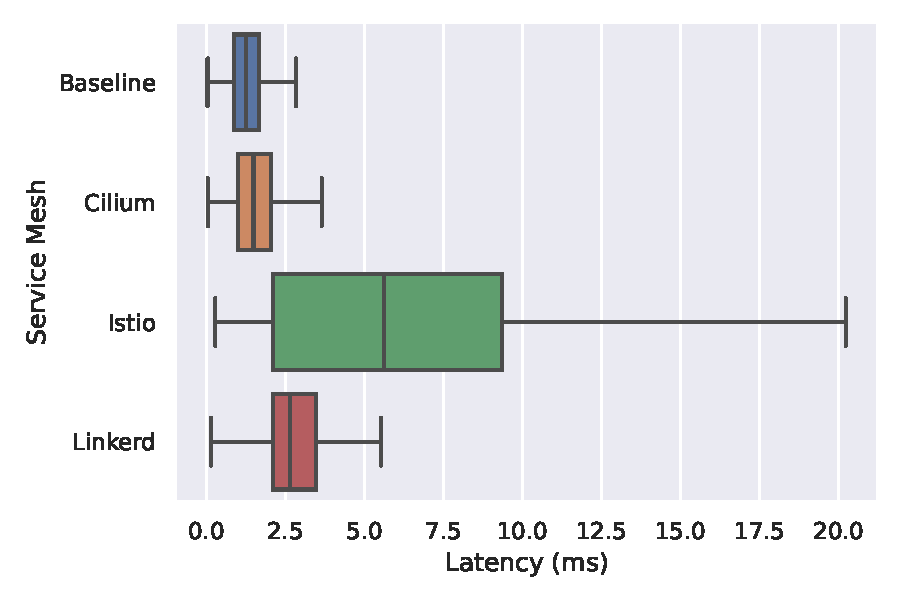
\includegraphics[width=\textwidth]{5_experimental_evaluation/figures/exp-01-latency-no-traefik.pdf}
      \caption{Linear scale, excluding Traefik}
      \label{fig:exp:01:boxplots-latency:linear}
    \end{subfigure}
}
\caption[Experiment 1 - Latency distributions of \gls{sm} systems under maximum load.]{Latency distributions of \gls{sm} systems under maximum load.}
\label{fig:exp:01:boxplots-latency}
\end{figure}


In \cref{fig:exp:01:boxplots-latency} we present a pair of box and whiskers plots that depict the locality, spread and skewness of latencies per \gls{sm} configuration. The lines at the borders of the box represent the 25th and 75h percentiles of data. The line in the middle of the box depicts the median observed value and the whiskers of the box represent the minimum and maximum values. It is important to note that the outliers are omitted from these figures, as we cover these in greater detail later on. The plots depicted in the figure share the meaning of their axes, where the y-axis represents the \gls{sm} configuration and the x-axis represent the observed latencies in milliseconds. The first plot (\cref{fig:exp:01:boxplots-latency:log}), shows all the \gls{sm} configurations and displays the box plots on a logarithmic scale. The second plot (\cref{fig:exp:01:boxplots-latency:linear}), displays the data on a linear scale but excludes Traefik.

In \cref{fig:exp:01:boxplots-latency:log} we present the observed latencies on a logarithmic scale. We do this because it shows that the observed latencies for Traefik surpass the other configurations by an order of magnitude. In \cref{fig:exp:01:boxplots-latency:linear} we compare the \gls{sm} configurations on a linear scale and exclude Traefik. From these results, we can observe that the distribution of observed latencies for Cilium is very similar to that of the baseline configuration. This indicates that the network overhead caused by the in-kernel proxy of Cilium is kept to a minimum which leads us to the third main finding:

\begin{shaded*}
    \noindent
    \textbf{MF3}: 
    The network latency overhead caused by the proxy of Cilium is minimal.
\end{shaded*}

Another observation we can make is that Linkerd has a slightly higher median and spread, but is still performing relatively well as it does not deviate too much from the baseline configuration. Istio, on the other hand, appears to suffer significantly more. Not only is the median affected, the spread of observed latencies is significantly greater. We can relate this behaviour to the type of proxy used in their data planes and their design decisions (see \cref{sec:survey:results} \cref{tab:result-proxy}). Whereas Istio uses \textit{Envoy}, a complex and feature rich general purpose proxy, Linkerd uses its own lightweight proxy \cite{linkerd-no-envoy}.


In \cref{fig:exp:01:tail-end-latencies} we present the tail end of latencies observed (above the 99th percentile) for the \gls{sm} configurations excluding Traefik. On the y-axis we represent the latencies observed in millisecond whereas the x-axis represents the various \gls{sm} configurations. The colours of the bars represent a certain percentile of latencies observed.

From the chart in \cref{fig:exp:01:tail-end-latencies} we can observe that Istio suffers the most in the observed tail end latencies. We observed a latency values of 40, 141 and 358 milliseconds for the 99th, 99.9th and 99.99th percentiles respectively. This observation is a continuation from the behaviour depicted in the box and whiskers plot (\cref{fig:exp:01:boxplots-latency:linear}), where the results tied to the configuration using Istio also depicted a large spread in observed latency values. This leads to a fourth main finding:

\begin{shaded*}
    \noindent
    \textbf{MF4}: 
    The latencies observed from Istio under load have a large spread, and especially suffer in their tail end.
\end{shaded*}

\begin{figure}[t]
\centering
\makebox[\linewidth][c]{
    \begin{subfigure}{.65\textwidth}
      \centering
      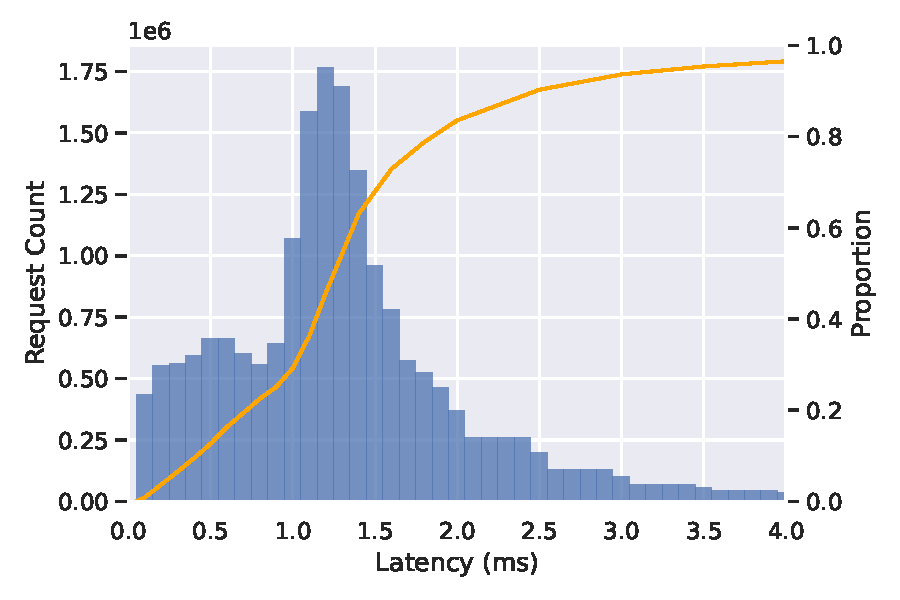
\includegraphics[width=\textwidth]{5_experimental_evaluation/figures/exp-01-latency-distribution-baseline.pdf}
      \caption{Baseline}
      \label{fig:exp:01:histogram:baseline}
    \end{subfigure}
    
    
    \begin{subfigure}{.65\textwidth}
      \centering
      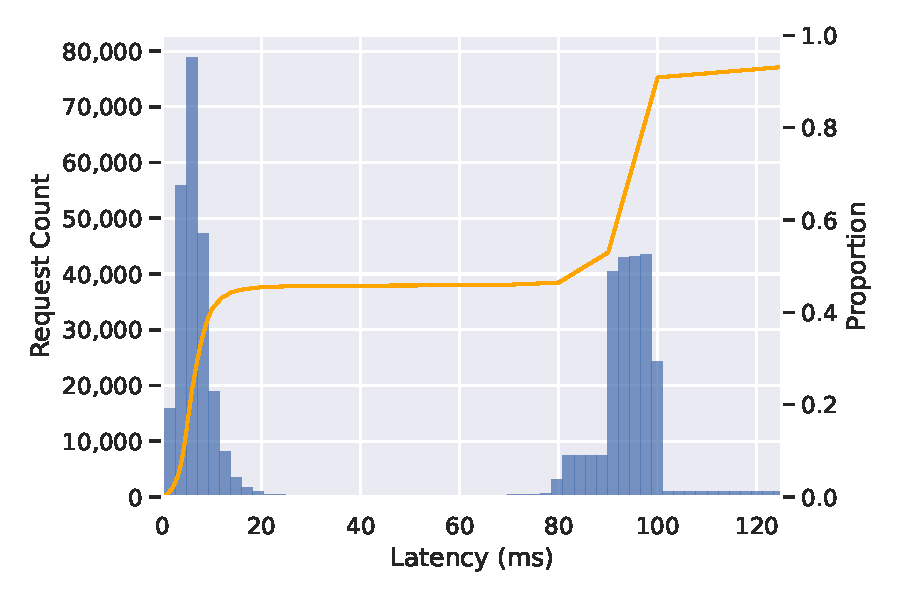
\includegraphics[width=\textwidth]{5_experimental_evaluation/figures/exp-01-latency-distribution-traefik.pdf}
      \caption{Traefik}
      \label{fig:exp:01:histogram:traefik}
    \end{subfigure}
}
\caption[Histogram of observed latencies under maximum load]{Histogram of observed latencies under maximum load per \gls{sm} configuration.}
\label{fig:exp:01:histograms-latency}
\end{figure}

To evaluate the behaviour of Traefik in more detail, we depict the latency distributions in a histogram. In \cref{fig:exp:01:histograms-latency} we depict two plots where each plot contains a histogram of latency distributions. The first plot contains the histogram of the baseline configuration (\cref{{fig:exp:01:histogram:baseline}}) and the second plot contains the histogram of Traefik  (\cref{{fig:exp:01:histogram:traefik}}). Each histogram has a y-axis that represents the number of requests for a specific bin and an x-axis that represents the latency in milliseconds. In addition to the bins, we depict the cumulative density function that shows the proportion of requests smaller than the latency depicted on the x-axis. 

From the results depicted in \cref{fig:exp:01:histograms-latency}, we can observe the distribution of latencies for the baseline configuration and that of Traefik. Note that the values next to the y-axis depict different values, there are more latencies observed for the baseline configuration, as the throughput was not fixed in this experiment. The shape of the distribution for the baseline configuration is similar to that of other configurations except for Traefik (see Appendix for a full comparison). From the shape of the histogram distribution of Traefik we can derive a peculiar finding, it has a bimodal distribution. The first mode is close to 8ms, whereas the second mode is around the 90 milliseconds. These observations lead to our fifth  finding of the experiment: 

\begin{shaded*}
    \noindent
    \textbf{MF5}: 
    Traefik mesh performs an order of magnitude worse than any other evaluated service mesh in terms of request latencies when the system is under full load.
\end{shaded*}

\subsubsection{Resource Utilization Analysis}
\label{sec:experiments:results:per-experiment:01:resource}


\begin{figure}[t]
\centering
\makebox[\linewidth][c]{
    \begin{subfigure}{.65\textwidth}
      \centering
      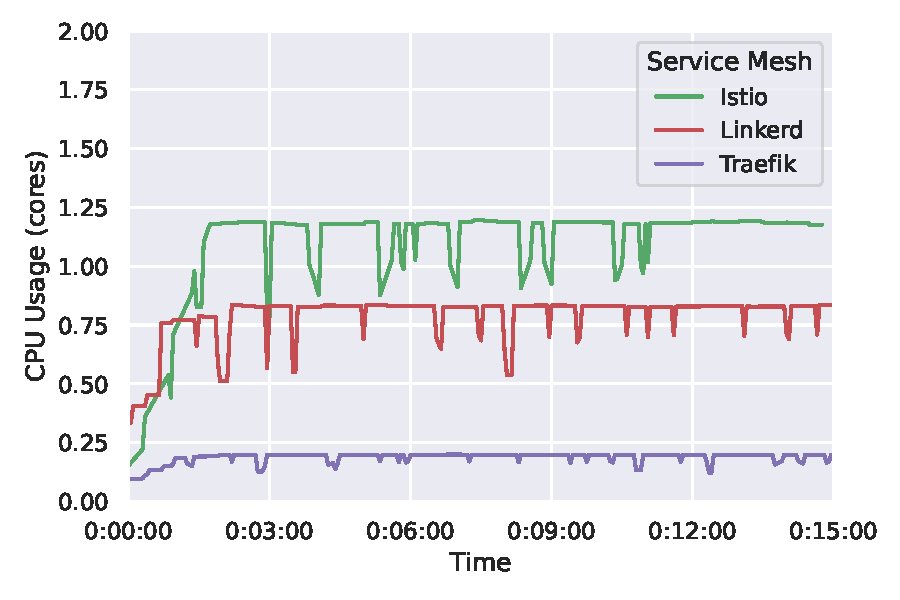
\includegraphics[width=\textwidth]{5_experimental_evaluation/figures/exp-01-cpu-utilization.pdf}
      \caption{CPU Utilization}
      \label{fig:exp:01:resource:cpu}
    \end{subfigure}
    
    
    \begin{subfigure}{.65\textwidth}
      \centering
      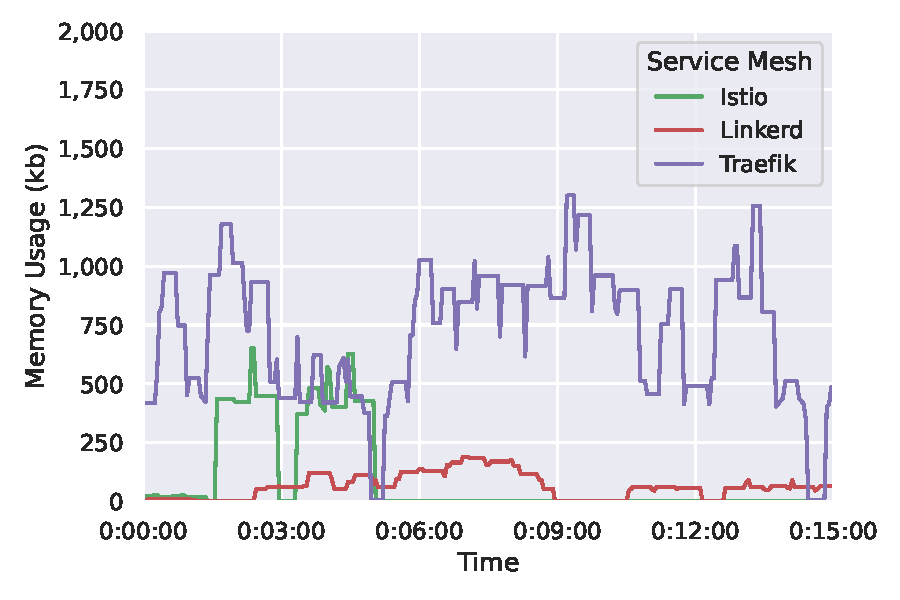
\includegraphics[width=\textwidth]{5_experimental_evaluation/figures/exp-01-memory-utilization.pdf}
      \caption{Memory Utilization}
      \label{fig:exp:01:resource:mem}
    \end{subfigure}
}
\caption[Experiment 1 - Resource utilization for \gls{sm} systems under load.]{Resource utilization for \gls{sm} systems under load.}
\label{fig:exp:01:resource-utilization}
\end{figure}


The final type of analysis that we perform is related to the utilization of system resources. In \cref{fig:exp:01:resource-utilization}, we present two line graphs that depict resource usage over time. The first plot (\cref{fig:exp:01:resource:cpu}) is related to the CPU utilization of \gls{sm} proxies. The y-axis represents the fraction of CPU cores used for the \gls{sm} proxy (on a two core system), and the x-axis represents the time delta of the experiment. The second plot depicts \cref{fig:exp:01:resource:mem} the memory utilization. For this, plot the y-axis represents the memory utilization in kilobytes, whereas the x-axis once again represents the time delta of the experiment. In these plots, we display three out of four \gls{sm} systems. This is because we were only able to capture the user-level application containers related to Cilium, and not the kernel-level proxy. For this reason, we omit Cilium from the resource graphs, as the data gathered was inconclusive for that system.

The results as depicted in \cref{fig:exp:01:resource-utilization} show the various configurations under varying levels of load. This means that the comparison cannot be considered fair. With that said, we can still observe some interesting behaviour. In \cref{fig:exp:01:resource:cpu} we depict the CPU utilization for the three observed systems. We can see that the proxy of Istio is the largest consumer of the CPU, even though as previously observed, it had a significantly fewer requests to process compared to Linkerd. This can be related to the aforementioned design decisions of the proxy implementations \cite{linkerd-no-envoy}. Another thing to note is that Traefik, the worst performing \gls{sm} system consumes the least amount of CPU resources. This at the very least proves that the poor performance is not related to any CPU related bottlenecks.

From the results depicting memory utilization (\cref{fig:exp:01:resource:cpu}) we can derive that the memory utilization for the data plane proxies is very minimal, even under maximum load. The highest values observed as depicted by the spikes in the graph, are less than 1500Kb and pose no significant bottleneck for most systems and environments.


\subsection{\ref{exp:design:2} - HTTP Constant Throughput}
\label{sec:experiments:results:per-experiment:02}
% Goal: To evaluate how \gls{sm} configurations behave under varying levels of load.

In the previous experiment (\cref{sec:experiments:results:per-experiment:01}), we evaluated \gls{sm} systems under maximum load. In this experiment, we evaluate these systems under varying, pre-defined levels of constant throughput. The results of these experiments aim to show how the \gls{sm} systems scale, across varying levels of load.

\subsubsection{Latency Analysis}
\label{sec:experiments:results:per-experiment:02:latency}

\begin{figure}[!t]
    \centering
    
    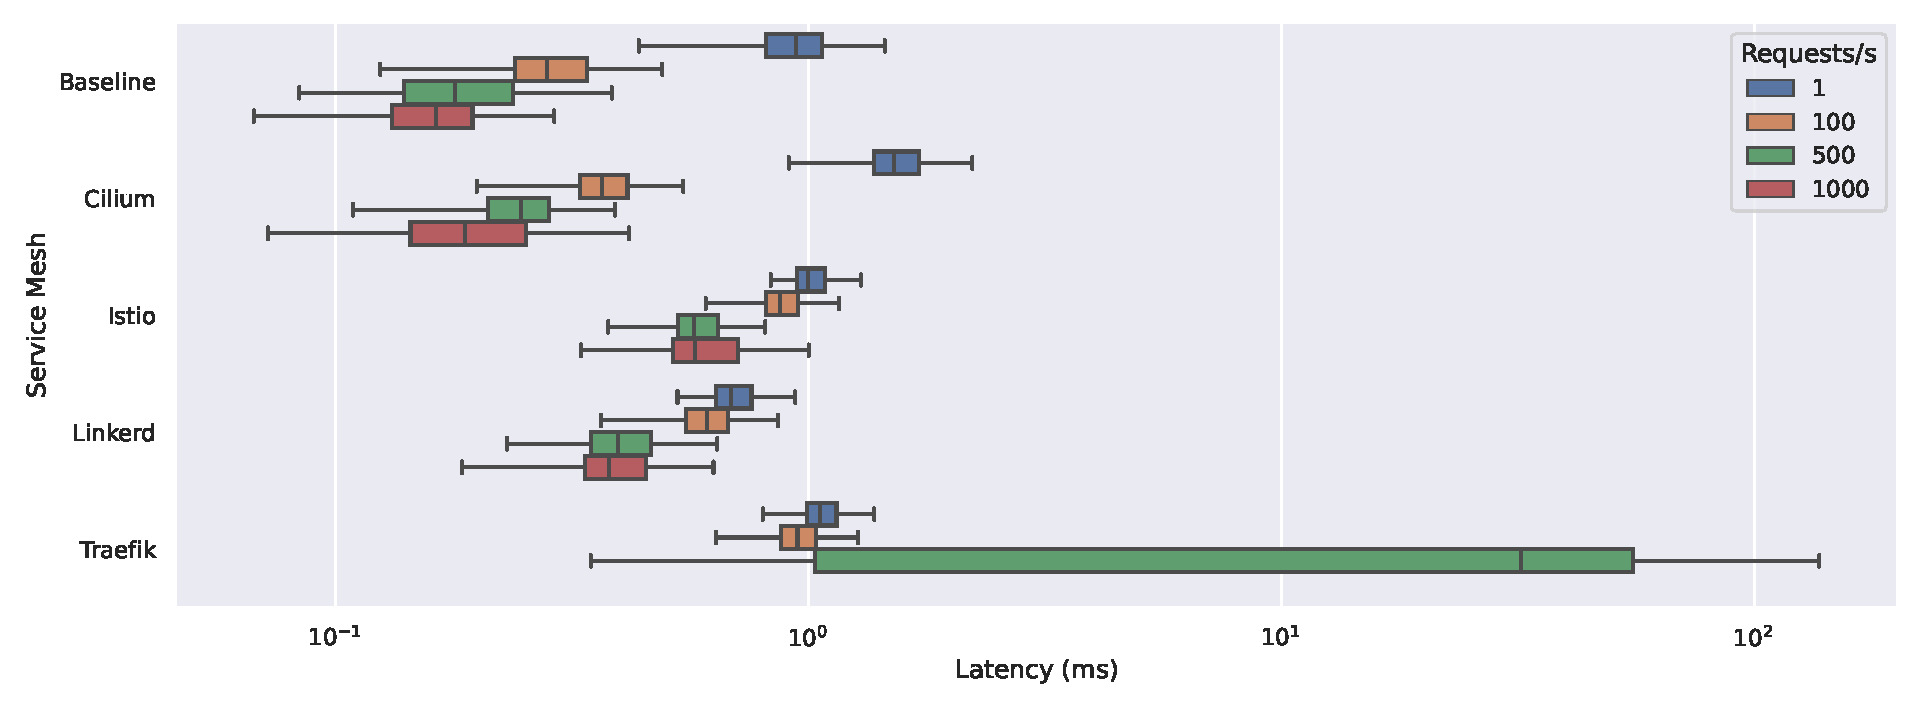
\includegraphics[width=1\linewidth]{5_experimental_evaluation/figures/exp-02-latency-log.pdf}
    
    \caption[Distribution of observed latencies per \gls{sm} system under various levels of constant throughput]{Distribution of observed latencies per \gls{sm} system under various levels of constant throughput on a logarithmic scale.}
    
    \label{fig:exp:02:latency-distributions}
\end{figure}


In \label{fig:exp:02:latency-distributions} we present the latency distributions of the evaluated \gls{sm} configurations under various levels of constant throughput.  On the y-axis we present the \gls{sm} configurations and on the x-axis the latency expressed in milliseconds on a logarithmic scale. The legend on the plots display the various levels of throughput depicted on this graph and the colours that represent them.

From the figure we can derive that the latency distributions are generally close for each of the defined levels of throughput for most of the systems. This is an indication that the various levels of throughput are manageable by the evaluated configurations. This is exemplified by the average levels of throughput that these configurations were able to process as observed in our previous experiment in \cref{sec:experiments:results:per-experiment:01}. 

One exception to this, however, is that the configuration using Traefik is experiencing a significant increase in observed latencies when experiencing a constant load of 500 requests per second. Additionally, it is important to note that the results regarding 1000 requests per second have not been included in this figure, as it was unable to manage that level of throughput. As a matter of fact, it was unable to even fully sustain the constant throughput of 500 requests per second, as it only managed to process 419 requests per second in this particular experiment. This result falls in line with the observed behaviour from our previously conducted experiment, in which we evaluated these systems under maximum load. The reason that the observed throughput is even lower in this experiment compared to the previous one, is that the previous experiment allowed for dynamic levels of throughput. This experiment on the other hand, uses constant levels of throughput as generated by the workload generator. The workload generator, however, does not make up or increase the level of throughput to compensate if the system was unable to previously process the results in time. 

Additionally, we analysed the tail end latencies of the evaluated configurations under these levels of constant throughput. The results that depict these high percentile latencies can be found in the Appendix (\cref{fig:exp:02:tail-latencies}). However, at these levels of load, we did not observe any increase in high percentile latencies as we previously did in our first experiment. The values we observed for the constant levels of throughput align with the expected values of a normal distribution.

\subsubsection{Traefik Bottleneck Analysis}
\label{sec:experiments:results:per-experiment:02:traefik-bottleneck}

To provide a more extensive analysis into the observed behaviour of Traefik, we visualized the latency distributions of the configuration using Traefik in violin plot as depicted in \cref{fig:exp:02:traefik-bottleneck}. The y-axis of this plot represents the various levels of throughput, and the x-axis present the observed latency values in milliseconds. It is important to note that we did include the results of when we evaluated Traefik under a constant throughput of 1000 requests per second, even if it did not manage to actually sustain this level of throughput as previously discussed. 

\begin{figure}[!t]
    \centering
    
    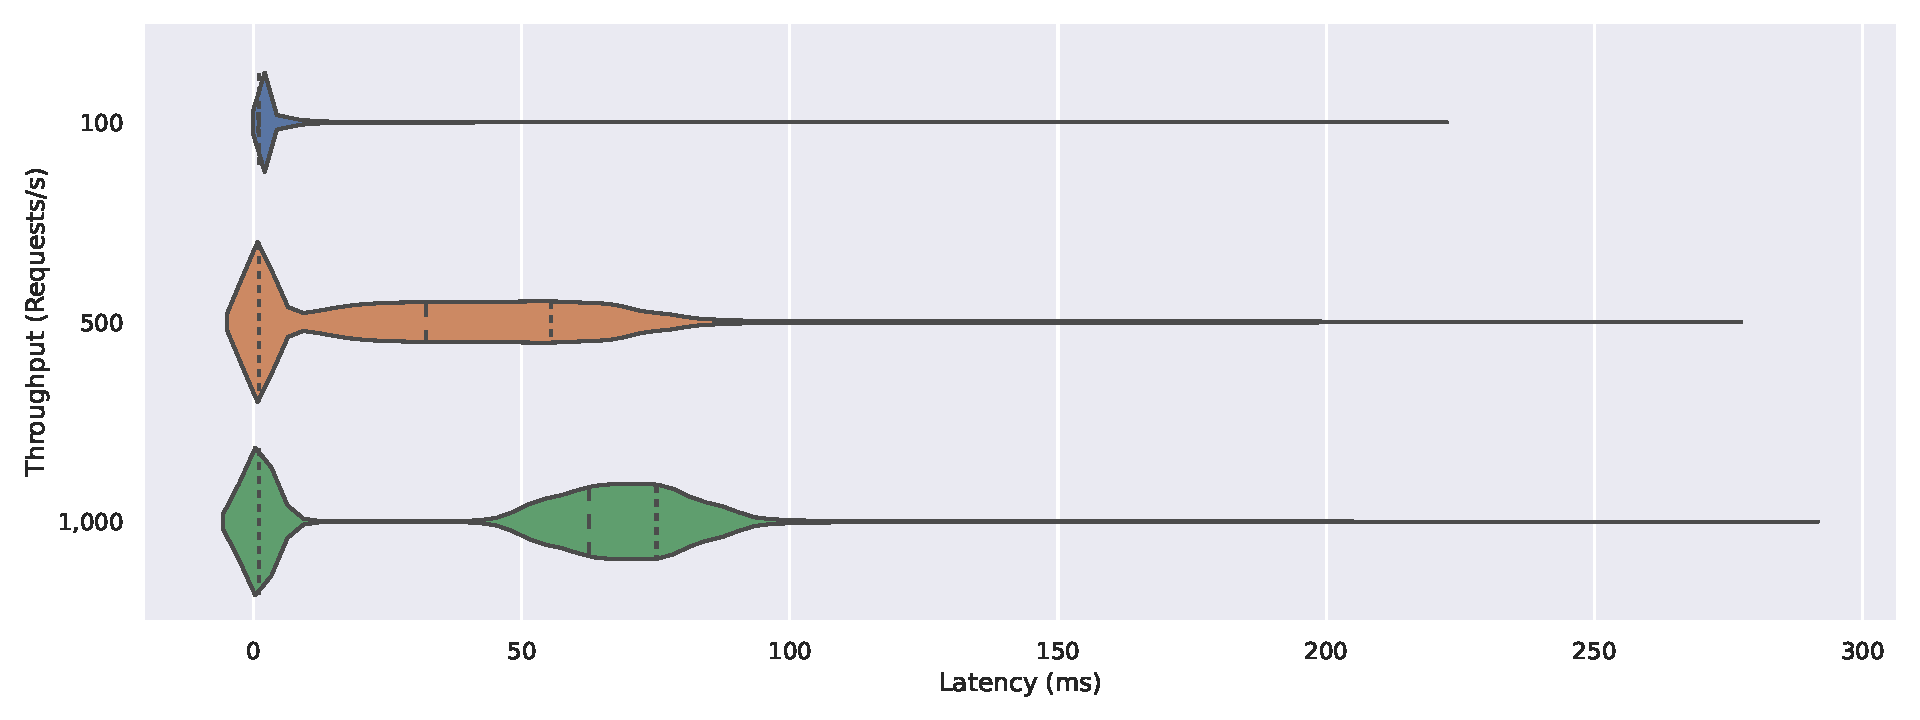
\includegraphics[width=1\linewidth]{5_experimental_evaluation/figures/exp-02-bottleneck-traefik.pdf}

    \caption[Latency distribution of Traefik under varying levels of constant throughput]{Latency distribution of Traefik under varying levels of constant throughput.}
    
    \label{fig:exp:02:traefik-bottleneck}
\end{figure}

Through the violin plots as depicted in \cref{fig:exp:02:traefik-bottleneck}, we can observe the behaviour and bottlenecks of the system under load in more detail. The first violin plot shows the latency distribution when it is under a constant load of 100 requests per second. From this, we can derive that the system can process this amount and that the distribution of latencies is similar to that of other evaluated \gls{sm} systems as previously seen. The second violin plot, however, shows the system under a constant load of 500 requests per second. This plot shows the first signals of a potential bottleneck in the system. We can observe that the observed latency values have a higher spread and that these values are often an order of magnitude higher, often reaching values well above 50 milliseconds. This provides a sharp contrast with the other systems that we evaluated, which performed significantly better under full or near full load. The third violin plot, however, shows the bottleneck in full effect. This plot depicts the system under a constant throughput of 1000 requests per second, which it was unable to process. This results in the previously observed bimodal distribution of requests latencies. This leads us to our sixth main finding:


\begin{shaded*}
    \noindent
    \ref{exp:mf6}: 
    Traefik experiences bottlenecking behaviour under a load of approximately 500 requests per second resulting in a bimodal distribution of request latencies.
\end{shaded*}


\subsubsection{Resource Utilization Analysis}
\label{sec:experiments:results:per-experiment:02:resource}

\begin{figure}
\centering
\makebox[\linewidth][c]{
    \begin{subfigure}{.6\textwidth}
      \centering
      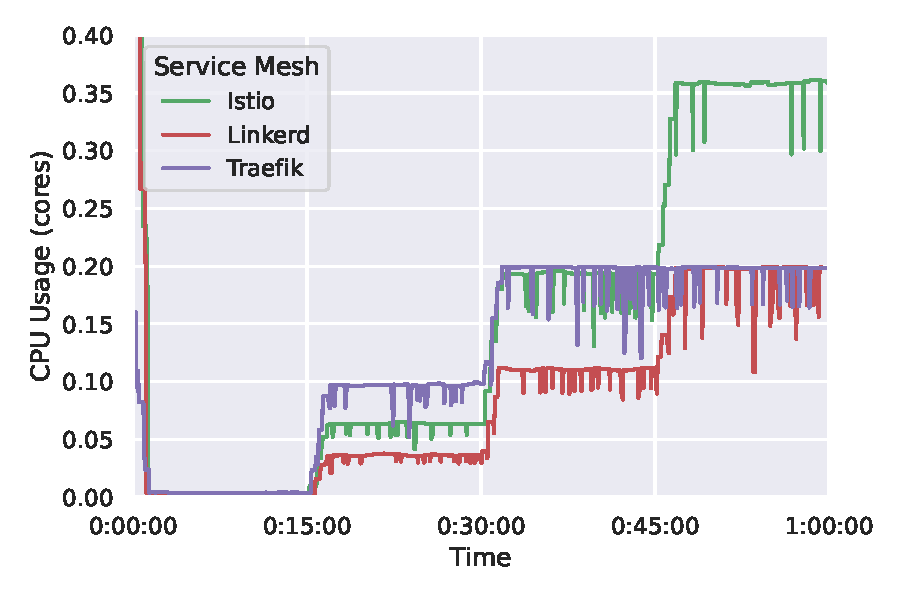
\includegraphics[width=\textwidth]{5_experimental_evaluation/figures/exp-02-cpu-utilization.pdf}
      \caption{CPU Utilization}
      \label{fig:exp:02:resource:cpu}
    \end{subfigure}
    
    
    \begin{subfigure}{.6\textwidth}
      \centering
      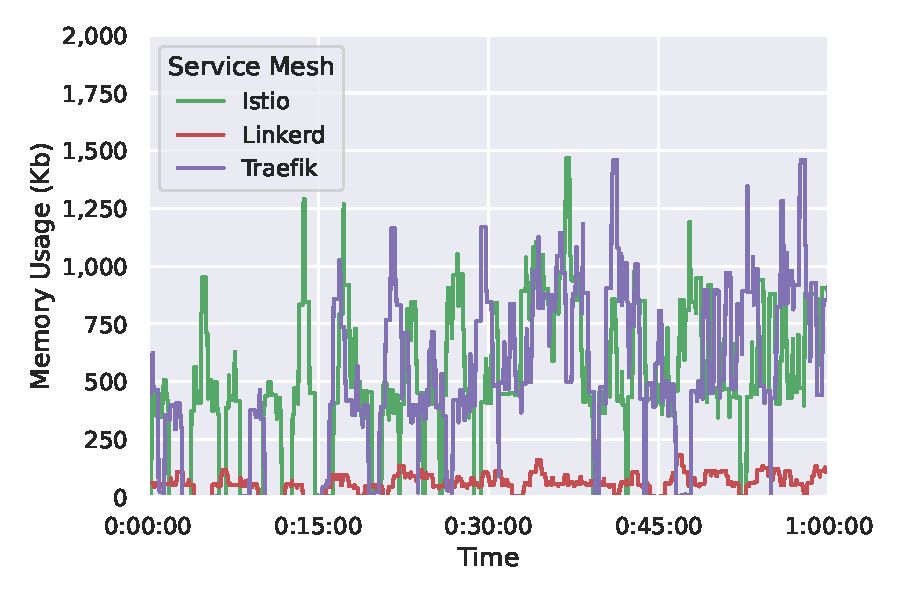
\includegraphics[width=\textwidth]{5_experimental_evaluation/figures/exp-02-memory-utilization.pdf}
      \caption{Memory Utilization}
      \label{fig:exp:02:resource:mem}
    \end{subfigure}
}
\caption[Resource utilization for \gls{sm} systems under load]{Resource utilization for \gls{sm} systems experiencing various levels of constant throughput. The level of throughput is increased at a 15-minute interval, and changes from  1, 100, 500, and 1000 requests per second respectively.}
\label{fig:exp:02:resource-utilization}
\end{figure}

In our first experiment we already took a look at the resource utilization values of various \gls{sm} systems under maximum load. However, those results could not be compared fairly, as they each experienced various levels of load. In this experiment, however, we can evaluate the resource utilization fairly as they are evaluated under similar circumstances. 

In \cref{fig:exp:02:resource-utilization} we present two plots related to the resource consumption of \gls{sm} systems. Both plots can be interpreted similarly. On the y-axis we have the value of interest, which is the CPU utilization as expressed in fractions of a core for the first plot and is the memory utilization expressed in Kb for the second plot. The x-axis presents the time delta of the experiment since the start. It is important to note the labels on the x-axis as these 15-minute intervals represent the time point in which the level of constant throughput was increased. The four intervals represent the constant levels of throughput from 1, 100, 500, and 1000 requests per second respectively (e.g. the interval from 0:30:00 to 0:45:00 represents the systems under a constant load of 500 requests per second). Additionally, the colours of the line represent the various \gls{sm} systems that we evaluated. As previously noted, we are unable to evaluate the actual resource utilization of Cilium as the actual in-kernel proxy is not exposed as a user-space application in the form of a container.

The first plot (\cref{fig:exp:02:resource:cpu}), shows the CPU utilization throughout the experiment for the various \gls{sm} systems. The first thing we can observe the high values at the start of the experiment, these can be explained by the sampling rate used for the time series data which overlaps with the results from the previous experiment. The second thing we can notice is that the line from Traefik does not increase at the 45:00 minute marker. This behaviour falls in line with the previously discussed bottlenecks in our extensive analysis of the bottlenecks of Traefik. Another observation that we can make is that the CPU utilization is relatively stable for all the evaluated systems throughout the duration of the experiment, we can derive this from the lack of extremes and spikes in the presented plot.

More importantly, however, we can observe how the systems scale when the load on these systems is increased. By looking at the first 15-minute interval, we can observe that the proxies require little to no CPU utilization when they experience next to zero load (1 request per second). Interestingly however, is the behaviour when the load is increased to 100 requests per second as it allows us to fairly compare these systems under a similar load. We can observe that the Traefik proxy utilizes the CPU the most, whereas the proxy in the Istio data plane requires just slightly more than half of Traefik's usage. The Linkerd proxy, however, puts the least amount of strain on the CPU requiring less than 5\% of a CPU core at any given time. To analyse how these systems scale we take a closer look at the third and final time intervals. From this, we can observe that the CPU utilization scales linearly with the levels of throughput that a proxy is facing. We can also observe that the proxy empowering the Linkerd \gls{sm} scales significantly better than the one found in Istio. This is exemplified by the fact that Istio under a load of 500 requests per second uses nearly identical amount of CPU resources when Linkerd serves double the number of requests per second. This leads us to a seventh main finding:

\begin{shaded*}
    \noindent
    \ref{exp:mf7}: 
    There can be a significant difference in the amount of CPU utilization for different \gls{sm} systems under similar levels of load.
\end{shaded*}

The second plot (\cref{fig:exp:02:resource:mem}), shows the CPU utilization throughout the experiment for the various \gls{sm} systems. The first observation that we can make is that the amount of memory consumed for all systems does not seem to vary much across the various levels of throughput. Furthermore, we can observe that the linkerd proxy consumes the least amount of memory whereas Traefik and Istio's data plane proxy seem to consume similar amounts. More importantly, however, is that all the observed values are negligible for most environments. This brings us to our eighth main finding:

\begin{shaded*}
    \noindent
    \ref{exp:mf8}: 
    The memory footprint of data plane proxies is negligible and does not significantly increase under higher levels of throughput.
\end{shaded*}


\subsection{\ref{exp:design:3} - HTTP Payload}
\label{sec:experiments:results:per-experiment:03}


\subsection{\ref{exp:design:4} - gRPC Maximum Throughput}
\label{sec:experiments:results:per-experiment:04}
% Goal: To evaluate how meshed configurations behave with alternative communication protocols.

In the final experiment we utilize a different type of application workload. In the previous experiments we evaluated the different configurations and \gls{sm} systems using various HTTP workloads. In this experiment, we use a different application level protocol to evaluate how the layer-7 aware data plane proxies perform with alternative layer-7 application protocols. 



\begin{figure}[ht]
\centering
\makebox[\linewidth][c]{
    \begin{minipage}{.65\textwidth}
      \centering
      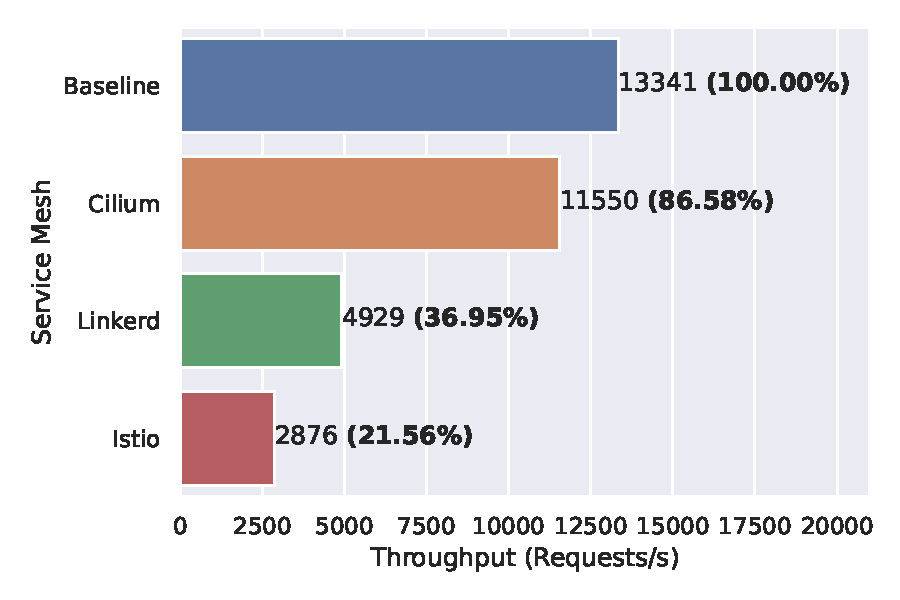
\includegraphics[width=\linewidth]{5_experimental_evaluation/figures/exp-04-max-throughput.pdf}
      \caption[Average throughput of \gls{sm} systems under maximum load using the gRPC protocol]{Average throughput of \gls{sm} systems under maximum load using the gRPC protocol.\\}
      \label{fig:exp:04:maximum-throughput}
    \end{minipage}
    
    
    \begin{minipage}{.65\textwidth}
      \centering
      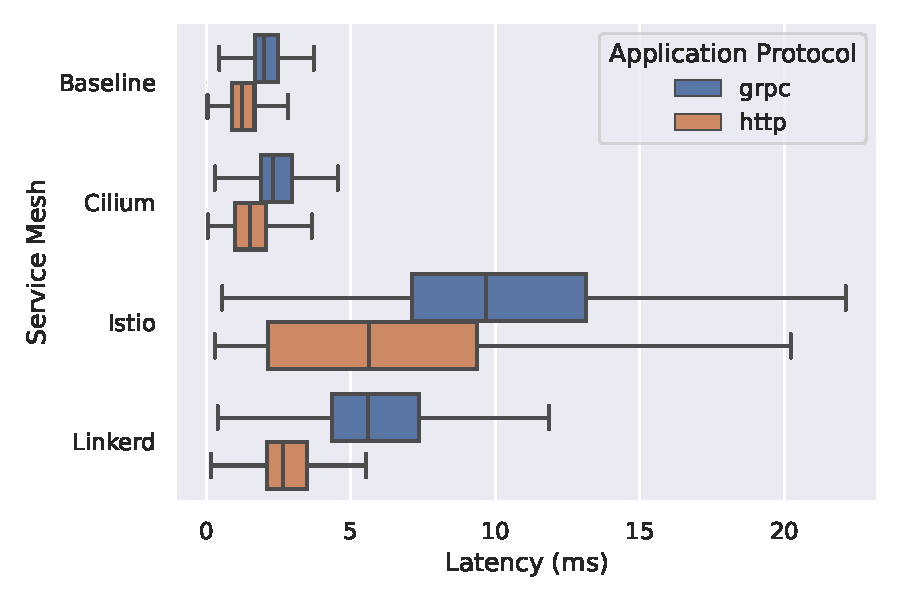
\includegraphics[width=\linewidth]{5_experimental_evaluation/figures/exp-04-latency-compared.pdf} 
      \caption[Comparing the latency distributions of \gls{sm} systems under maximum load for both HTTP and gRPC workloads]{Comparing the latency distributions of \gls{sm} systems under maximum load for both HTTP and gRPC workloads.}
      \label{fig:exp:04:latencies-compared}
    \end{minipage}
}
\end{figure}


\subsubsection{Maximum Sustained Throughput Analysis}
\label{sec:experiments:results:per-experiment:04:throughput}

In \cref{fig:exp:04:maximum-throughput} we present a bar chart which depicts the average throughput a \gls{sm} system was able to process throughout the 15-minute duration of the experiment. During this experiment, the workload generator produced as many requests as the receiving system was able to process and did so in an unrestricted manner. The results are presented in the chart which can be interpreted as follows. On the y-axis we present the different \gls{sm} configurations. The x-axis presents the aggregated average throughput value that a configuration was able to process, expressed in requests per second. The values next to the bars represent the actual observed value and the percentage next to it represents the percentage of throughput a system was able to process compared to the best performing configuration, which in this case is the baseline.


The very first thing to notice in \cref{fig:exp:04:maximum-throughput} is the absence of Traefik in the depicted chart. This is because the proxy in Traefik was unable to process any gRPC requests and any attempt in doing so resulted in errors even though historical articles produced by the vendor explicitly state the support for the gRPC protocol \cite{maesh-introduction}. This leads to our tenth main finding:

\begin{shaded*}
    \noindent
    \textbf{MF10}:
    The configuration using Traefik was unable to process any gRPC based requests.
\end{shaded*}

% Comparison of HTTP vs gRPC (reduction of throughput)
% Cilium $16.83\%$ $13.42\%$
% Linkerd $54.94\%$ $63.05\%$ 
% Istio $80.09\%$ $78.44\%$
% Traefik $97.39\%$  - 

Another observation we can make is regarding the levels of throughput a \gls{sm} system can process compared to the baseline configuration. Similarly to the first experiment, in which we evaluated the maximum sustained throughput whilst using HTTP-based requests and responses (\cref{sec:experiments:results:per-experiment:01}), we observe that there is a significant reduction of throughput for each of the evaluated \gls{sm} systems. The best performing \gls{sm} system is once again, Cilium, experiencing a $13.42\%$ reduction in throughput compared to the baseline configuration. Linkerd is the second best performing system, which experiences a $63.05\%$ reduction. The greatest reduction of throughput, however, is reserved for the Istio which experiences a massive $78.44\%$ reduction in throughput compared to the baseline.

When we compare these results to the results from the first experiment we can observe a similar trend. We observe the same ranking whilst evaluating this metric. Additionally, the relative differences when comparing the reductions per protocol are minimal. Most of the evaluated systems experience similar reductions for both application level protocols. The largest difference observed is for Linkerd, which encountered a $54.94\%$ reduction for the HTTP workloads whilst it encountered a $63.05\%$ reduction for the gRPC based workloads. This brings us to our eleventh main finding:

\begin{shaded*}
    \noindent
    \textbf{MF11}:
    Both gRPC and HTTP-based workloads experience similar reductions in terms of sustained throughput.
\end{shaded*}

\subsubsection{Latency Analysis}
\label{sec:experiments:results:per-experiment:04:latency}


In \cref{fig:exp:04:latencies-compared} we present the latency distributions of the evaluated configurations under maximum load for both the gRPC and HTTP-based workload experiments. On the y-axis we present the evaluated configurations, excluding Traefik. On the x-axis we present the latency in milliseconds. The colours of the bar indicate the type of workload used. The blue bars (gRPC) present the data from the fourth experiment, whereas the orange bars (HTTP) present the observed latency values from the first experiment.


\begin{figure}[ht]
\centering
\makebox[\linewidth][c]{
    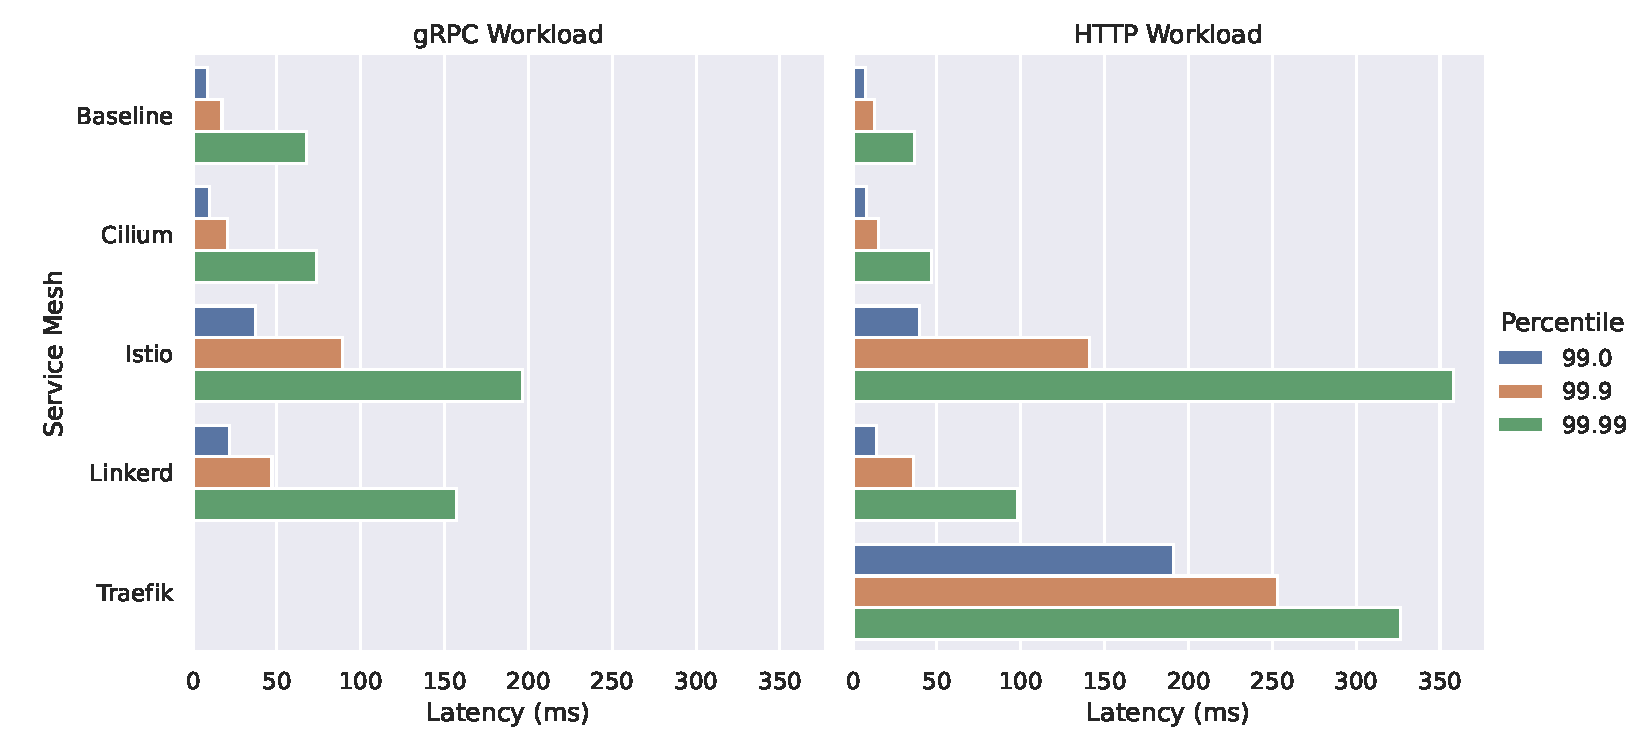
\includegraphics[width=1.3\linewidth]{5_experimental_evaluation/figures/exp-04-tail-latencies-all-compared.pdf} 
}

   \caption[Tail end latencies of \gls{sm} systems experiencing maximum load per application protocol]{Tail end latencies of \gls{sm} systems experiencing maximum load per application protocol.}
    
   \label{fig:exp:04:tail-latencies}

\end{figure}

The first observation that we can make is that the observed latency values are slightly higher for the gRPC based workloads across all the evaluated configurations. Furthermore, we can observe that the spread of latency values for Linkerd is larger when using a gRPC-based workload, compared to the HTTP-based counterpart. Although there are some differences, we can conclude that there are no significant differences in the latency distributions based on the application protocol.


In \cref{fig:exp:04:tail-latencies} take a closer look at the observed tail end latencies for both types of application level protocols used. On the y-axis we present the evaluated \gls{sm} configurations and on the x-axis we present the latency in milliseconds. Within the plots we depict coloured bars, in which the colours represent the 99th, 99,9th, and 99.99th percentile respectively. The plot on the left displays the results for the gRPC-based workload whereas the plot on the right presents the result for the HTTP-based workload.

From the plots as depicted in \cref{fig:exp:04:tail-latencies} we can observe a couple of interesting findings. First, we observe that the tail end latencies, specifically the 99.99th percentile are negatively affected whilst using the gRPC based protocol for the baseline configuration and the configurations using Cilium and Linkerd. Interestingly however, is that the tail end latencies of Istio improved significantly when exposed to gRPC-based workloads compared to the HTTP counterpart. This could be related to the manner in which the data plane proxy, Envoy, processes gRPC based requests as they treat is as a first class citizen at both the transport and application layer\footnote{\url{https://www.envoyproxy.io/docs/envoy/latest/intro/arch_overview/other_protocols/grpc}}.



\section{Summary}
\label{sec:experiments:summary}


